\documentclass{article}
\usepackage{tikz}
\usetikzlibrary{automata,positioning}

\begin{document}

\begin{figure}[h]
    \centering
    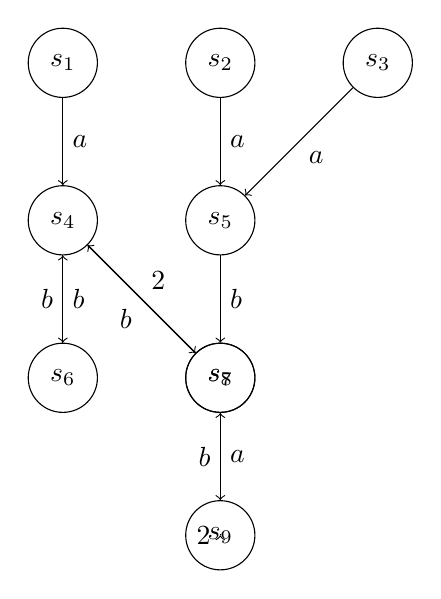
\begin{tikzpicture}[node distance=2cm, auto]
        % States
        \node[state] (s1) {$s_1$};
        \node[state] (s2) [right of=s1] {$s_2$};
        \node[state] (s3) [right of=s2] {$s_3$};
        \node[state] (s4) [below of=s1] {$s_4$};
        \node[state] (s5) [below of=s2] {$s_5$};
        \node[state] (s6) [below of=s4] {$s_6$};
        \node[state] (s7) [below of=s5] {$s_7$};
        \node[state] (s8) [right of=s6] {$s_8$};
        \node[state] (s9) [below of=s8] {$s_9$};

        % Edges
        \path[->]
            (s1) edge node {$a$} (s4)
            (s2) edge node {$a$} (s5)
            (s3) edge node {$a$} (s5)
            (s4) edge node {$b$} (s6)
            (s4) edge node {$2$} (s7)
            (s5) edge node {$b$} (s7)
            (s6) edge node {$b$} (s4)
            (s7) edge node {$b$} (s4)
            (s8) edge node {$a$} (s9)
            (s9) edge node {$2$} (s9)
            (s9) edge node {$b$} (s8);
    \end{tikzpicture}
    \caption{Sample Transition Diagram}
    \label{fig:sample_diagram}
\end{figure}

\end{document}